\graphicspath{{}{theory/}{Diagrams/}}

This chapter is dedicated to studying some important and more technical aspects of neutrino physics for the rest of the thesis. We start by reviewing some of the most popular models to explain non-zero neutrino masses beyond the SM. This will be useful to introduce neutrino masses and mixing, with which we can comment on neutrino oscillations in vacuum and in matter. We then move on to discuss the usual approach to studying neutrinos in the laboratory, focusing on accelerator experiments. We will find that it is hard to ignore the strong force in many of the most important neutrino cross sections.

%%%%%%%%%%%%%%%%%%%%%%%%%%%%%%%%%%%%%%%%%%%%%%%%%%%%%%%%%%%%%%%%
%
% MASS MODELS
%
%%%%%%%%%%%%%%%%%%%%%%%%%%%%%%%%%%%%%%%%%%%%%%%%%%%%%%%%%%%%%%%%%%

\section{Mass Mechanisms}

Understanding the theoretical origins of neutrino mass and mixing is a worthwhile but ambitious task. The possibilities are endless and the high-scale dynamics, typical of many neutrino mass models, is hard to test in the laboratory. Presently, it is fair to say there are more neutrino mass models than ways to test them. Nonetheless, many of these models possess similar features and just a couple of low energy observables are sufficient to probe a large class of models. These models may rely on the seesaw mechanism, on radiative effects or in extended scalar sectors. On top of that, new symmetries and fundamental forces may also be at play, making the theories more predictive. We will now explore a small fraction of this model space.

We have already alluded to the first possibility to introduce light neutrino masses in the SM. All that is needed are at least two RH neutrino fields, singlets under all SM symmetries. We shall refer to them as $N^\alpha$, where $\alpha$ is their generation index. This may be chosen to be $\alpha = e, \mu, \tau$ or any combination of two of these. The full new neutrino mass Lagrangian then becomes
%
\begin{equation}\label{eq:typeILagrangian}
 \mathscr{L}_{\nu-{\rm mass}} = \overline{N}^\alpha i\slashed{\partial} N_\alpha - y^\nu_{\alpha\beta} \left( \overline{L}^\alpha \widetilde{H} \right) N^\beta - \left(y^\nu_{\alpha\beta}\right)^* \overline{N^\beta} \left( \widetilde{H}^T  L^\alpha\right)  - M_{\alpha \beta} \overline{N^c}^\alpha N^\beta,
\end{equation}
%
where $N^c = C \overline{N}^T$ with $C$ the charge conjugation matrix ($C = i \gamma^2 \gamma^0$ in the Dirac and Weyl representation). The middle terms endow neutrinos with Dirac masses, but the last one is a new ingredient. This is the Majorana mass matrix for the new RH neutrinos, and it is allowed by the symmetries of the model. It does, however, violate any $U(1)$ symmetry associated with the fields $N$, as
%
\begin{equation}
 N \to e^{i\theta} N \,\implies\, \overline{N^c} N \to e^{2i\theta}\overline{N^c} N.
\end{equation}
%
So if $N$ are assigned lepton number, then the accidental global symmetries of the SM $B-L$ and $L$ are violated by the Majorana mass term. If we insist and set $L(N)=0$, then the Dirac mass term will, instead, explicitly break these global symmetries. This interesting observation, together with the fact that gauging $B-L$ leads to an anomaly-free theory with three RH neutrinos, has led proposals of Dirac neutrino mass models with gauged and unbroken $B-L$~\cite{Heeck:2014zfa}. On top of that, the scale of the entries in $\textbf{M}$ is not set by the Higgs vev and, therefore, may be wildly different from the EW scale. We may argue that it has to be small, since in the limit that all $M_{\alpha\beta}\to0$, the SM symmetry is enhanced and the theory is said to be technically natural in the t'Hooft sense. Regardless of our argument to prevent this term, one thing is clear, a purely Dirac neutrino mass model has to deal with the fact that the neutrino Yukawas are extremely small $y^\nu/y^t \approx 10^{-12}$. If the arbitrariness of Yukawa couplings in the SM already made us uncomfortable, this SM extension dramatically worsens the picture. Of course, we may be tempted to ignore the flavour puzzle and just stop here. This solution, however, as underwhelming as it is, is not unique. Many other models for neutrino masses exist and, while we cannot rule all of them out, it is worthwhile to study the alternatives.

In the same way that the $N$ particles admitted a Majorana mass term, we may wonder if the SM may also provide a similar term for the LH states. Clearly $SU(2) \times U(1)$ invariance forbids any renormalizable operator that would give rise to this operator before SSB, but at $d=5$, we can write the so-called Weinberg operator
%
\begin{equation}\label{eq:weinberg}
 \mathscr{L}_{d=5} = \frac{c_{\alpha\beta}}{\Lambda} \left( \overline{L^c} \widetilde{H}^* \right) \left( \widetilde{H}^\dagger L  \right) \to  \frac{c_{\alpha\beta}}{\Lambda} \frac{v^2}{2} \overline{\nu_L^c}^\alpha \nu_L^\beta
\end{equation}
%
where we go from the unbroken to the broken phase. This operator is, in fact, the only $d=5$ operators allowed in the SM effective field theory (SMEFT). The fact that the lowest dimension non-renormalizable operator in the SMEFT gives neutrino masses is, yet again, another indication that neutrino masses point towards BSM physics. Unfortunately, assuming the coefficients to be $\mathcal{O}(1)$ and saturating the upper bound on the sum of neutrino masses $m_\nu \lesssim 0.1 $ eV, we are led to conclude that $\Lambda \approx 10^{14}$ GeV, eerily close to the Planck scale. There is, however, no reason to expect the couplings of the theory to be large and for the mass mechanism to be simple. Technical naturalness, for instance, is commonly invoked to claim that the mass mechanism may reside at low scales, where we trade unreachable energies for tiny couplings. We will shortly see all tree-level UV-completions to the Weinberg operator. Of course, neutrino masses need not be tree-level effects, and loop-induced mechanisms for generating Dirac or Majorana neutrino masses are also important. In this case, the smallness of neutrino masses is explained through loop suppression factors. We come back to these issues in \refsec{sec:seesaws}.


The mass term induced by \refeq{eq:weinberg} turn out to be of the Majorana kind. Testing this hypothesis is extremely difficult because of the smallness of $m_\nu$. Any process containing lepton number violation (LNV), the hallmark of Majorana neutrinos, will be suppressed by $m_\nu^2/E^2$, where $E$ is the typical energy involved. Another way to understand this is that any process where the operator above is important must be sensitive to the effects of neutrino mass, which we have yet to measure. Curiously, this holds also for neutrino oscillations. In that case, one might also worry about additional phases that appear in the Majorana case, but these can be shown to drop out. Currently, the most promising search for the Majorana nature of neutrinos is neutrinoless double-beta decay ($0\nu\beta\beta$), $(A,Z)\to(A,Z+2) + e^- + e^-$. This process is only allowed if neutrinos are Majorana, and should be contrasted with double-beta decays ($2\nu\beta\beta$), where two neutrinos are present in the final state.  



\subsection{Conventional Seesaw Mechanisms}\label{sec:seesaws}

There exist only three ways to UV complete the Weinberg operator at tree-level. These correspond to introducing a new fermion which is a singlet of $SU(2)_L$, a new scalar that transforms as a triplet of $SU(2)_L$ or a new fermion that also transforms as a triplet. These models are usually referred to as the Type I~\cite{Minkowski:1977sc,Mohapatra:1979ia,Yanagida:1979as,GellMann:1980vs}, Type II~\cite{Konetschny:1977bn,Cheng:1980qt,Lazarides:1980nt,Schechter:1980gr,Mohapatra:1980yp} and Type III~\cite{Foot:1988aq} seesaw mechanism, respectively. They are shown in \reffig{fig:seesaw_mechanisms} and we discuss each one individually below.
%
\begin{figure}[t]
\centering
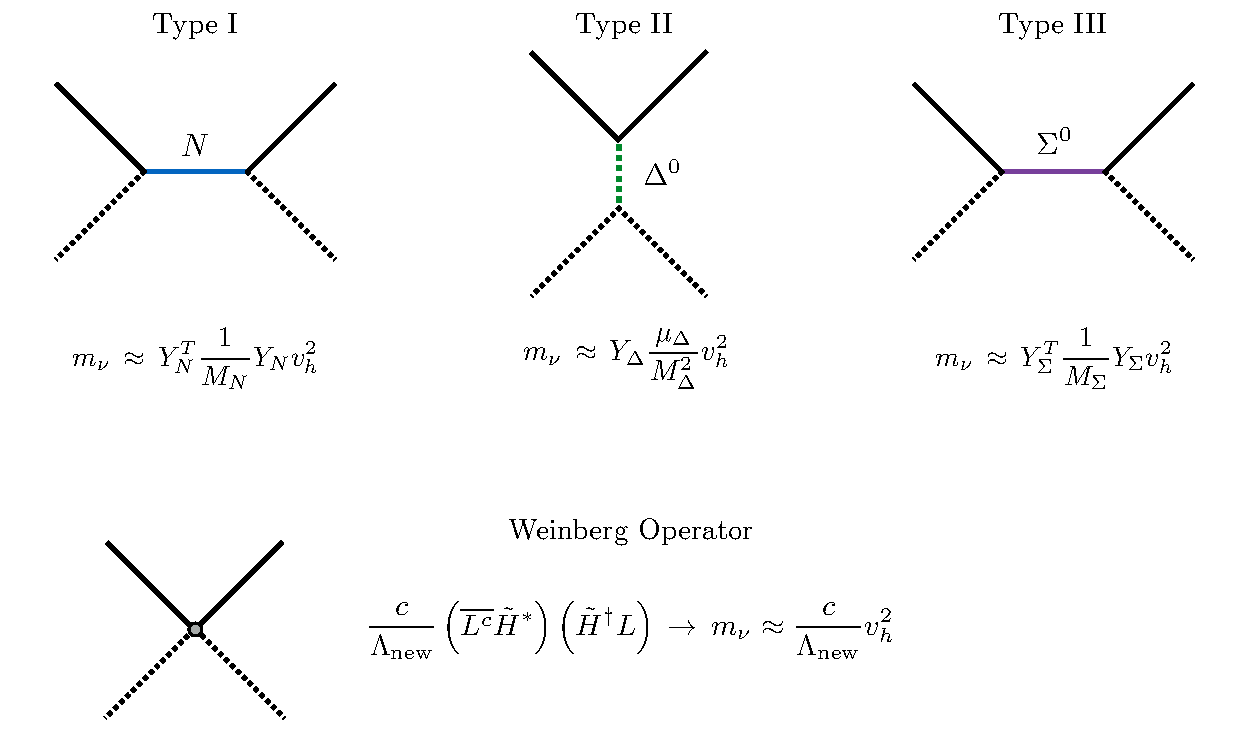
\includegraphics[width=\textwidth]{seesaw_mechanisms.pdf}
\caption[The tree-level UV completions of the Weinberg operator.]{The tree-level UV completions (top) of the $d=5$ Weinberg operator (bottom) with their respective contributions to light neutrino masses.\label{fig:seesaw_mechanisms}}
\end{figure}
%


\paragraph{Type I} The Lagrangian for this extension is precisely the one in \refeq{eq:typeILagrangian}. For convenience, let us work in the single generation case. We collect all mass terms into a single mass matrix of the form
%
\renewcommand{\arraystretch}{0.8}
\begin{equation}
  -\mathscr{L}_{\nu-{\rm mass}} \supset \frac{1}{2} \left( \begin{matrix}  \overline{\nu_L} & \overline{N^c} \end{matrix} \right) \left( \begin{matrix}  0 &  m \\ m & M_N \end{matrix} \right)  \left( \begin{matrix} \nu_L^c \\ N \end{matrix} \right) \,+\, {\rm h.c.},
\end{equation}
%
where $m = y^\nu_N v/\sqrt{2}$ and $M_N$ is the Majorana mass for $N$. Diagonalizing this mass matrix with a simple rotation $R(\theta)$, we find
%
\begin{equation}
 m_{1,2} = \frac{M_N \pm \sqrt{M_N^2 - 4m^2}}{2},\quad {\rm with}  \quad\tan{2 \theta} = \frac{2 m}{M_N}.
\end{equation}
%
In the so-called seesaw limit ($m \ll M_N$), this simplifies to 
%
\begin{equation}
 m_{1} \approx -\frac{m^2}{M_N} = \frac{(y^\nu_N v)^2}{2 M_N}, \quad m_2 \approx M_N  \quad {\rm with}, \quad \theta \approx \frac{m}{M_N},
\end{equation}
%
where the seesaw mechanism is in action: the large separation of scales between $m$ and $M_N$ explains the smallness of the light neutrino masses $m_1$. Saturating the upper bound on neutrino masses $m_1 \approx 0.1$ eV, we can infer that
\begin{equation}
 \left(y^\nu_N\right)^2 \approx 3 \times 10^{-15} \, \left(\frac{M_N}{{\rm GeV}} \right), \qquad \theta^2 \approx 10^{-10} \, \left(\frac{M_N}{{\rm GeV}} \right)^{-1}.
\end{equation}
%
Again, we conclude that the scale of new physics for couplings of $\mathcal{O}(1)$ lies at $M_N \approx 10^{15}$ GeV, in this case with very small mixing angles between the light states and the flavour $N$. Of course, this is only a naive scaling and becomes more complicated in the full three generation case~\cite{Casas:2001sr}. Nevertheless, it shows that heavy neutrinos at reasonably low scales are a reachable candidate to realise the seesaw mechanism, provided we are comfortable with small values for $y^\nu_N$.

\paragraph{Type II} In the presence of a scalar $\bm{\Delta}$, triplet under $SU(2)$, we can write
%
\begin{equation}\label{eq:typeIILagrangian}
 - \mathscr{L}_{\nu-{\rm mass}} \supset y^\nu_\Delta \, \overline{L^c} i\sigma_2 \bm\Delta L, \quad {\rm with}\quad \bm{\Delta} = \left( \begin{matrix} \Delta^+/\sqrt{2} & \Delta^{++} \\ \Delta^0 & -\Delta^+/\sqrt{2} \end{matrix} \right),
\end{equation}
%
where new charged scalars are appear. The scalar potential acquires the term
\begin{equation}
 -V(H,\Delta) \supset  \mu_\Delta H^T \,i\sigma_2\bm{\Delta} H + M_\Delta^2 \Tr{\bm{\Delta}^\dagger\bm{\Delta}},
\end{equation}
%
and is in general much more complicated. One can show that the neutral component acquires a vev $\langle \Delta^0 \rangle \approx \mu_\Delta v^2/M_\Delta^2$, where we ignored additional mixing terms between the Higgs and the new scalar degrees of freedom~\cite{Arhrib:2011uy}. This vev, then gives neutrinos mass through \refeq{eq:typeIILagrangian}, which interestingly, is linear in the neutrino Yukawa and suppressed by the typical mass scale of $\Delta$
%
\begin{equation}
 m_1 \approx y^\nu_\Delta  \frac{\mu_\Delta \,v^2}{M_\Delta^2}.
\end{equation}
%
The field $\bm{\Delta}$, in fact, carries lepton number $L=2$, and so the LNV parameter $\mu_\Delta$ being small is a technically natural choice. In this model, the vev of $\Delta^0$ is constrained to be very low, $\langle \Delta^0 \rangle \lesssim 5$ GeV, as $\bm{\Delta}$ contributes to the EW gauge boson masses through its kinetic term ${\rm Tr}\left[ (D_\mu \bm{\Delta})^\dagger (D^\mu\bm{\Delta}) \right]$. Finally, we can see for $m_1 \approx 0.1$ eV, we get
%
\begin{equation}
 y^\nu_\Delta \approx \left( \frac{1 {\rm eV}}{ \mu_\Delta}\right)  \, \left( \frac{M}{1 \,{\rm TeV}}\right)^2,
\end{equation}
%
suggesting a clear target for experimental searches around at EW scale.

\paragraph{Type III} The fermionic triplet couples to the doublets through
%
\begin{equation}\label{eq:TypeIII}
 - \mathscr{L}_{\nu-{\rm mass}} \supset y^\nu_\Sigma \, \overline{L} \bm{\Sigma} H, \quad {\rm with } \quad 
\bm{\Sigma} = \left( \begin{matrix} \Sigma^0 &  \Sigma^+/\sqrt{2} \\ \Sigma^-/\sqrt{2} & - \Sigma^0 \end{matrix} \right).
\end{equation}
%
In this case, the scalar sector may remain unchanged and the field $\Sigma^0$ behaves very similarly to the field $N$ in the Type I seesaw. Analogously to the Type I, we can write 
%
\begin{equation}
 m_1 \approx \frac{(y^\nu_\Sigma v)^2}{2 M_\Sigma}.
\end{equation}
%
This model is much less explored in the literature, but its phenomenology is quite rich. The term related to charged-leptons in \refeq{eq:TypeIII} induces charged-lepton mixing, and leads to rare processes such as $\mu\to e\gamma $ and $\mu \to e e e $ already at tree-level, contrary to the Type-I seesaw where they appear at one loop.

\subsection{Low-Scale Seesaw Variants} All of the previous models may be searched for at low or high energy ranges, but for large Yukawa couplings, are regarded as high-scale solutions to the neutrino problem. Exceptions to this arise in constructions where additional symmetry arguments are at play. Most famous are the Inverse Seesaw (ISS)~\cite{Mohapatra:1986bd,GonzalezGarcia:1988rw} and the Linear Seesaw (LSS)~\cite{Wyler:1982dd,Akhmedov:1995ip,Akhmedov:1995vm}, where the lightness of neutrino masses is explained by an approximate conservation of lepton number, and the Extended Seesaw (ESS)~\cite{Kang:2006sn,Barry:2011wb,Zhang:2011vh}, where new hierarchies appear in the heavy sector. All these extensions arise from introducing additional neutral fermions to the Type I seesaw particle content. In particular, in the single generation case, the most general mass matrix we can construct with the new fermions $N$ and $S$ is given by~\cite{LopezPavon:2012zg}
%
\begin{equation} \label{eq:typeIvariants}
   -\mathscr{L}_{\nu-{\rm mass}} \supset \frac{1}{2} \left( \begin{matrix}  \overline{\nu_L} & \overline{N} &  \overline{S} \end{matrix} \right) \left( \begin{matrix}  0 &  m & \epsilon \\ m & \mu^\prime & \Lambda  \\ \epsilon & \Lambda & \mu \end{matrix} \right)  \left( \begin{matrix} \nu_L^c \\ N^c \\ S^c \end{matrix} \right) \,+\, {\rm h.c.}
\end{equation}
%
Note that lepton number, defined as $L = L_e + L_\mu+L_\tau+L_N+L_S$, is violated by $\mu$, $\mu^\prime$ and $\epsilon$ if we assign, as usual, $L_N = - L_S$. From the diagonalization of this mass matrix, we learn that 
\begin{equation}
 m_1 = \frac{\mu m^2 - 2 \epsilon m\Lambda  + \epsilon^2 \mu^\prime }{\Lambda^2 - \mu \mu^\prime}.
\end{equation}
%
Therefore, we see that if all LNV parameters are set to zero, neutrino masses vanish. In the same way, if we set $\epsilon,\mu \to 0$, then we also get vanishing neutrino masses, at tree level. This accidental cancellation is very peculiar, and will be realised in the model introduced in Chapter 5. As it turns out, $\mu^\prime$ breaks lepton number, and so radiative corrections can be large, responsible for the light neutrino masses in this case. 

The ISS model can be recovered in the limit $\Lambda \gg m \gg \mu \gg \mu^\prime, \epsilon$. Now, the smallness of neutrino masses are controlled by the LNV parameter $\mu$, which is small due to approximate conservation of $L$, and suppressed by $1/\Lambda^2$, realising the seesaw mechanism. In this way, the additional neutrino states combine into a pseudo-Dirac pair, with a mass of $m_{2,3} \approx \Lambda \mp (\mu+\mu^\prime)/2$. These type of models predict small LNV, but the new heavy fermions will reside at much smaller scales while mainting the Yukawa couplings large. The LSS is another special case where $\Lambda \gg m \gg \epsilon \gg \mu^\prime,\mu$. In this case the light neutrino mass is \emph{linear} in $m$ and suppressed by $\epsilon/\Lambda^2$. 


In the ESS limit, $\mu^\prime \gg \Lambda, m \gg \mu, \epsilon$, LNV is large and the light neutrino masses are suppressed by the scale $\mu^\prime$. The seesaw, in this case, happens both for light and intermediate neutrinos, and so light new fermions are typical predictions of the model, of interest to the literature on scale sterile neutrinos.

% These models have been extensively studied in the framework of Minimal Flavour Violation (MFV)~\cite{Gavela:2009cd}, where the only source of flavour violation is assumed to be equal to that in the SM (through Yukawa couplings). 
%
\begin{figure}[t]
\centering
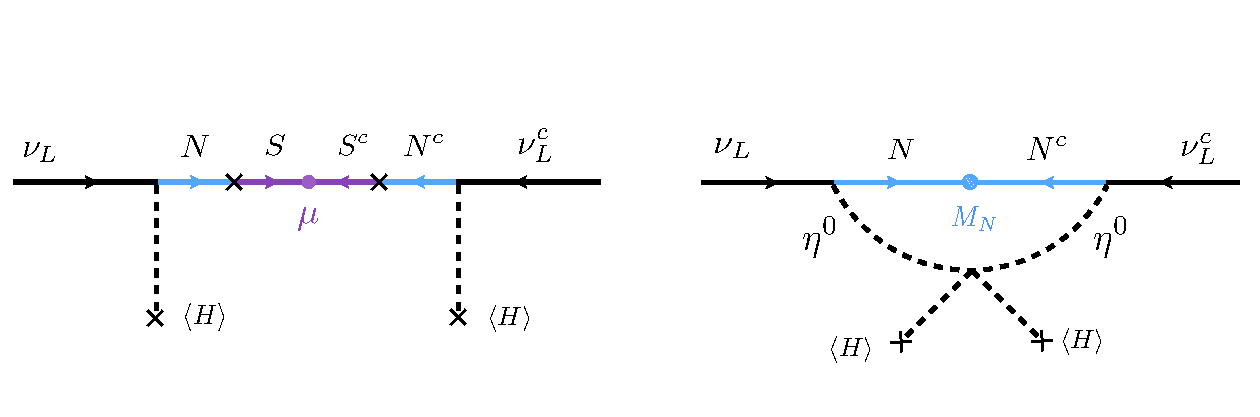
\includegraphics[width=\textwidth]{LNV_diagrams.pdf}
\caption[Diagrams for inverse seesaw and scotogenic model.]{On the left, the inverse seesaw flavour diagram for Majorana neutrino masses. On the right, the flavour diagram for the scotogenic mode. Arrows represent lepton number. \label{fig:LNVdiagrams}}
\end{figure}
%
\subsection{Radiative Masses}\label{sec:radiative}

A further possibility to generate the Weinberg operator is that Majorana neutrino masses arise from higher-order diagrams in perturbation theory. Since in the SM $L$ is an accidental symmetry, neutrino masses vanish at all orders, but this may not be the case in a generic SM extension. For instance, neutrino masses may arise at $n$ loops, in which case a naive estimate for the scale of new physics is
%
\begin{equation}
 \frac{c}{\Lambda} \approx  \left( \prod_{i}^\text{\# of vertices} g_i \right) \left(\frac{1}{4\pi}\right)^{2n} \frac{1}{M},
\end{equation}
%
where $g_i$ stand for the new couplings of the theory and $M$ is a new mass scale. The loop suppression factor is of interest since it lowers the scale $\Lambda$ without the need for small couplings or large masses. Many models for radiative neutrino masses exist, where typically new particles are introduced together with a new symmetry that prevents any of the mechanisms discussed previously to take place. 

The most illustrative example is perhaps the \emph{scotogenic} model~\cite{Ma:2006km}, sometimes also referred to as the radiative seesaw. Here, new SM singlet fermions $N$ are introduced together with $\eta$, a copy of the Higgs doublet with $\eta = (\eta^+, \eta^0\,)^T$ and $Y_\eta = Y_{H} = 1$. To forbid tree-level masses, an additional $Z_2$ discrete symmetry is introduced, under which all new states are odd ($N \to -N$ and $\eta \to -\eta$) and all SM particles are even (\eg, $L \to L$). In the single generation case, the new fermion mass terms are
%
\begin{equation}
-\mathscr{L}_{\nu-{\rm mass}} \supset \frac{M_N}{2} \overline{N^c} N + \left[y^N \left(\overline{L} \, \widetilde{\eta} \right) N \,+\, {\rm h.c.} \right],
\end{equation}
%
where the Yukawa term $(\overline{L} \widetilde{H}) N$ is not allowed by virtue of the $Z_2$ symmetry. The scalar potential now contains 
%
\begin{equation}
 V(H,\eta) \supset m_{\eta}^2 \eta^\dagger \eta + \frac{\lambda^\prime}{2} \left[ \left( H^\dagger \eta\right)^2 + \left( \eta^\dagger H \right)^2 \right],
\end{equation}
%
where $m_\eta^2 > 0$ and $\eta^0 = (\eta_R + i \eta_I)/\sqrt{2}$ acquires no vev. After SSB, we end up with an additional neutral scalar $\eta_R$ and neutral pseudo-scalar $\eta_I$ of masses $m_{R,\, I}^2 = m_\eta^2 \pm \lambda^\prime v^2/2$. The one-loop neutrino masses are then given by 
%
\begin{equation}
 m_1 = \frac{1}{2}\left(\frac{y^N}{4\pi}\right)^2 M_N \left[ \frac{m_R^2}{m_R^2 - M_N^2 } \ln \left( \frac{m_R^2}{M_N^2} \right) - \frac{m_I^2}{m_I^2 - M_N^2 } \ln \left( \frac{m_I^2}{M_N^2} \right) \right].
\end{equation}
%
In this case, we can see the loop suppression and the new Yukawas. To find what mass scale appears in the denominator, we may choose a limit. For $M_N \gg m_\eta$, we find $m_1 \propto \lambda^\prime v^2/M_N$ up to loop factors and the Yukawas, while for $M_N \ll m_\eta$, we have $m_1 \propto \lambda^\prime v^2 M_N/m_\eta^2$. The diagram on the right in \reffig{fig:LNVdiagrams} explicitly shows how this dependence comes about. 

Note that due to the $Z_2$ symmetry, $N$ and $\eta^0$ define a dark sector, with the lightest particle being a DM candidate. Despite the absence of the neutrino portal operator in this case, neutrino mixing between light states and the flavour $N$ is generated at one loop. In addition, the $\eta^\pm$ provides a strong connection between the SM and the dark sector. Many models for radiative neutrino masses display similar features to these, where new dark states often solve the neutrino and DM puzzle at the same time. This connection is explored in more detail in Chapter 5. Beyond one loop, neutrino mass models have been studied up to three-loop level~\cite{Krauss:2002px}.

\section{Neutrino Mixing} Now that we have a series of concrete models to generate neutrino masses, we would like to understand the consequences of massive neutrinos at low energies and how we learned about their mass. For our current purposes, we will focus purely on the $SU(2)$ breaking operator for Majorana and Dirac neutrino masses
%
\begin{equation}\label{eq:lowEmasses}
 \mathscr{L}_{\nu-{\rm mass}}^{\rm M} = \frac{M_{\alpha \beta}}{2} {\overline{\nu_L^c}^\alpha \nu_L^\beta} \,+\, {\rm h.c.,} \qquad %
 \mathscr{L}_{\nu-{\rm mass}}^{\rm D} = \frac{y^\nu_{\alpha \beta} v}{\sqrt{2}} \,{\overline{\nu_L}^\alpha N^\beta} \,+\, {\rm h.c.,}
\end{equation}
%
where the former Lagrangian describes purely Majorana neutrinos, and the latter describes purely Dirac neutrinos with the addition of three $N$ states to the SM. We will work with only three $N$ states for simplicity, any number greater than two is analogous. Similarly to the quark sector, we would like to diagonalize these mass matrices and find the relevant mixing matrix. We proceed with the two cases in parallel and start by rotating all fields independently with unitary matrices
%
\begin{align}
\nu_L^\alpha \to U^\nu_{\alpha k} \nu_L^k, \qquad & N^\alpha \to V^\nu_{\alpha k} N^k \nonumber\\
 e_L^\alpha \to U^e_{\alpha k} e_L^k,\qquad & e_R \to V^e_{\alpha k} e^k,
\end{align}
%
where $U$ ($V$) rotates LH (RH) fields. From \refeq{eq:lowEmasses}, it is clear that the diagonalization is slightly different in the two cases. The diagonal mass matrices are 
%
\begin{equation}
\textbf{M} \to \hat{\textbf{M}} = \textbf{U}^{\nu\,T} \textbf{M} \textbf{U}^\nu, \qquad   \textbf{Y} \to \hat{\textbf{Y}} = \textbf{U}^{\nu\,\dagger} \textbf{Y} \textbf{V}^\nu,
\end{equation}
%
where $\textbf{M}$ and $\textbf{Y}$ are diagonal matrices~\footnote{Note that in the Dirac case, the mass matrix $\textbf{Y}$ is diagonalized by its singular value decomposition, and in the Majorana case we assumed $\textbf{M}$ to be complex \emph{symmetric} and the special case of Takagi factorization applies.}. The CC Lagrangian defines lepton mixing through the Pontecorvo-Maki-Nakagawa-Sakata (PMNS) matrix~\cite{Pontecorvo:1957qd,Maki:1962mu}
%
\begin{equation}
\overline{e_L}^\alpha \gamma_\mu P_L \nu_L^\alpha \to \overline{e_L}^k P_L \, \left(U_{\rm PMNS}\right)_{kj} \,\nu_L^j, \qquad \textbf{U}_{\rm PMNS} = \textbf{U}^{e\,\dagger} \textbf{U}^\nu.
\end{equation}
%
At this point, we can identify the charged-lepton fields $e^k$ with their gauge basis (\ie, their flavour and mass basis coincide $\alpha \sim k$) and define the LH flavour neutrino field $\widehat{\nu}^\alpha = \left(U_{\rm PMNS}\right)_{\alpha j} \nu_L^j$. This is the relevant field for all neutrino CC interactions, but it does not have a well-defined mass. For simplicity, we will now adopt the notation $\widehat{\nu}^\alpha \equiv \nu^\alpha$.
%
\begin{figure}[t]
\centering
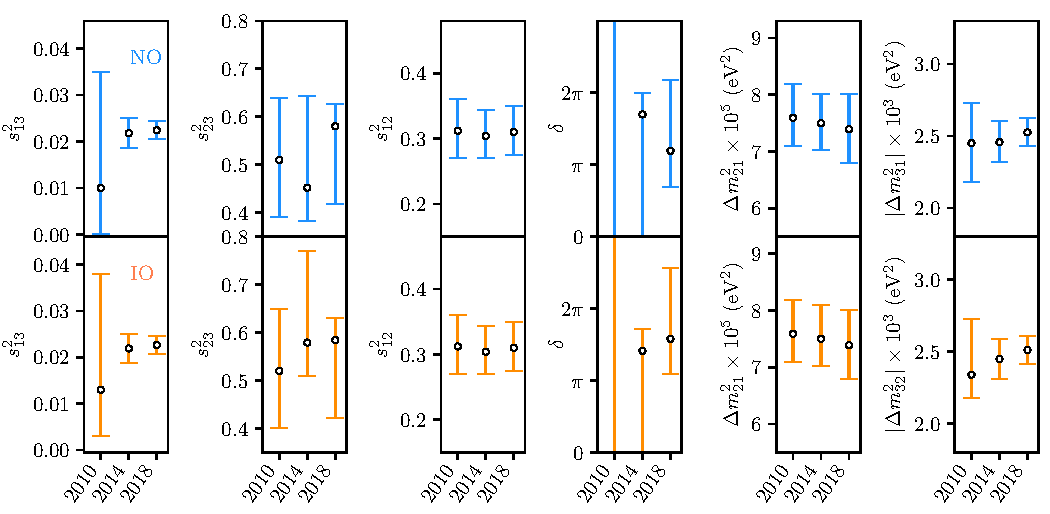
\includegraphics[width=\textwidth]{plots/precision2.pdf}
  \caption[Oscillation global-fit comparison between 2010, 2014 and 2018 datasets.]{The neutrino oscillation global-fit results in 2010~\cite{Schwetz:2011qt}, 2014~\cite{Gonzalez-Garcia:2014bfa} and 2018~\cite{Esteban:2018azc}. We show the best-fit point, together with the $3\sigma$ regions for normal ordering (NO) and inverted ordering (IO).\label{fig:measurements}}
\end{figure}
%

The PMNS mixing matrix is responsible for neutrino mixing and its entries are model dependent, arising from the flavour structure of the neutrino Yukawas and Majorana masses. In the general case, it is parametrized by
\renewcommand{\arraystretch}{0.9}
\begin{align}\label{eq:neu:UmixFull}
U_{\rm PMNS}&= \left(
\begin{matrix}
1 & 0        & 0\\
0 & c_{23}   & s_{23}\\
0 & -s_{23}  & c_{23}\\
\end{matrix}
\right)\hspace{-1ex}\left(
\begin{matrix}
c_{13}              & 0  & s_{13}e^{-i\delta} \\
0                   & 1  & 0                  \\
-s_{13}e^{-i\delta} & 0  & c_{13}             \\
\end{matrix}
\right)\hspace{-1ex}\left(
\begin{matrix}
c_{12}  & s_{12} & 0 \\
-s_{12} & c_{12} & 0 \\
0       & 0      & 1 \\
\end{matrix}
\right) D, 
% \hspace{-1ex}\left(
% \begin{matrix}
% 1               & 0                 & 0 \\
% 0               & e^{i\alpha_2/2} & 0 \\
% 0               & 0                 & e^{i\alpha_3 / 2}
% \end{matrix}
% \right),
% \nonumber\\
% &=\left(
% \begin{matrix}
% U_{e 1}& U_{e 2}  & U_{e 3}\\
% U_{\mu 1} & U_{\mu 2} & U_{\mu 3}\\
% U_{\tau 1} & U_{\tau 2} & U_{\tau 3}\\
% \end{matrix}
% \right),
\end{align}
%
where $c_{ij} = \cos{\theta_{ij}}$ and $s_{ij}= \sin{\theta_{ij}}$ are the cosine and sine of the mixing angles to be measured from oscillation data. The matrix $D = {\rm diag}\{1,e^{i\alpha_2/2}, e^{i\alpha_3/2}\}$ contains additional phases that are physical when neutrinos are Majorana. As we will see in the next section, oscillation data can shed light on all mixing angles, mass-squared differences $m^2_{ij} = m_i^2 - m_j^2$, and on the CP-violating phase $\delta$. Neutrino oscillations are insensitive, however, to any Majorana phases.

Immense efforts to measure all parameters in the PMNS have been carried out in the past 26 years. In \reffig{fig:measurements}, we show the relative precision reported by a global-fit to neutrino oscillation data, comparing the data release from after the Neutrino conferences of 2010~\cite{Schwetz:2011qt}, 2014~\cite{Gonzalez-Garcia:2014bfa} and 2018~\cite{Esteban:2018azc}. All three mixing angles and two mass-squared splittings have been succesfully measured to at least $3\sigma$, with the exception of the CP-violating phase $\delta$, which is still largely unknown. Another interesting development is our knowledge of the mass ordering. This is a measurement of the sign of $\Delta m^2_{3\ell}$, where $\ell = 1$ for normal ordering (NO) and $\ell = 2$ for inverted ordering (IO). While currently the global-fit in Ref.~\cite{Esteban:2018azc} displays a mild preference for NO ($\Delta \chi^2 = 4.7$), future measurements are needed. For $\Delta m^2_{21}$, this sign is known, as it strongly impacts the matter potential of solar neutrinos.


\subsection{Neutrino Oscillations}

Neutrino oscillations arise when a superposition of neutrino mass eigenstates is produced, propagates macroscopic distances and scatters inside a detector. Given sufficiently long baselines, neutrino flavour transitions may always occurs due to mixing, but for a non-trivial dependence on baseline distances, coherence must be preserved throughout the process. In this section, we will make these statements more precise and derive the standard formula for the oscillation probability $P(\nu_\alpha \to \nu_\beta)$ in vacuum (matter effects are discussed in \refsec{sec:matter_effects}). This exercise can be done in multiple ways and most often derivations rely on plane-wave neutrino states. This approach leads to correct expressions for $P(\nu_\alpha \to \nu_\beta)$ in virtually all cases of interest, but it is a rather poor conceptual description of oscillations and relies on unphysical assumptions. Instead, we will derive the oscillation formula from a quantum mechanical wave packet approach, and encounter a few conditions for oscillations to happen. More sophisticated treatments in Quantum Field Theory (QFT), often called the \emph{external} wave packet approach, have been known for some time~\cite{Cardall:1999ze,Beuthe:2001rc,Giunti:2002xg}, and their results have been shown to be directly mapped onto the \emph{internal} wave packet approach~\cite{Akhmedov:2010ms} we discuss here. Nonetheless, neutrino oscillations are notorious for being conceptually confusing and the correct method to compute such processes is still debated in the literature~\cite{Kobach:2017osm}. We may seek consolation in the fact that a few aspects are common to all approaches, for instance, the ultra-relativistic nature of the mass states through expansions of $\sqrt{m^2 + p^2}$ and the need for momentum uncertainties in the initial and final neutrino processes.
%
\begin{figure}[t]
\centering
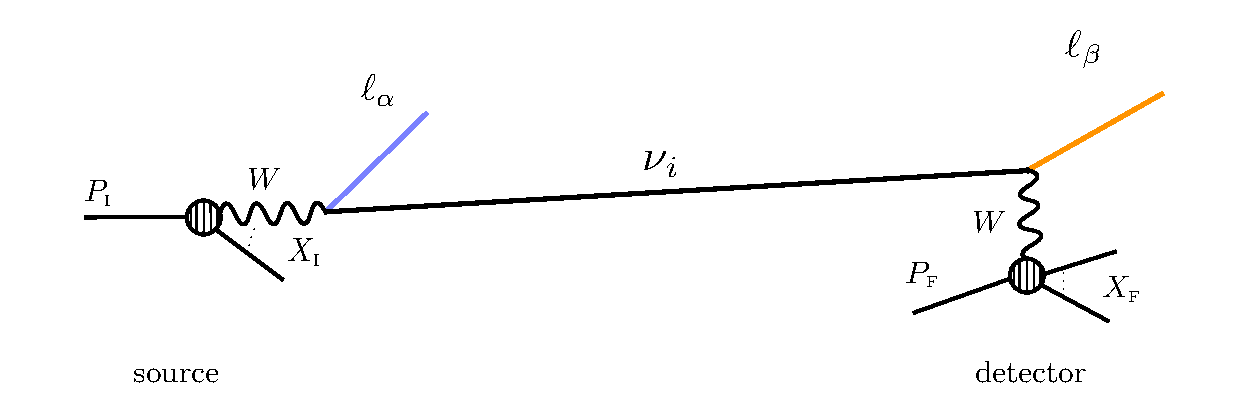
\includegraphics[width=\textwidth]{oscillations_diagram.pdf}
  \caption[Neutrino oscillations diagram.]{The usual set-up of an oscillation experiment. We show the source, where a process $P_\textsc{i} \to \nu_\alpha \, X_\textsc{i}$ happens (note that $P_\textsc{i}= \ell_\alpha$ is allowed and that $P_\textsc{i}$ may be a scattering process), and the detector, where $\nu_\beta \,P_i \to \ell_\beta \,X_\text{f}$. \label{fig:oscillations_diagram}}
\end{figure}
%

Our setup typical of neutrino oscillations experiments and is represented in \reffig{fig:oscillations_diagram}. We will first discuss the role of production and detection processes, and then later study the oscillations \emph{per se}. Initially, a neutrino flavour state $\nu_\beta$ is produced in a CC reaction at the source, $P_\textsc{i} \to \nu_\beta X_\textsc{i}$. More precisely, a state $\ket{f}$ is produced,
%
\begin{equation}\label{eq:flavour_source}
 \ket{f} = \hat{S} \ket{P_\textsc{i}}, \quad \hat{S} \approx  \hat{1} - i \int \dd^4 x \, H_{\rm int}^{\rm CC} (x),
\end{equation}
%
where $\hat{S}$ is the S-matrix operator approximated to first order in weak coupling and
%
\begin{equation}
 H_{\rm int}^{\rm CC} (x) = \sqrt{2} G_F\, \sum_\alpha \overline{\nu}_\alpha (x) \gamma^\mu P_L \ell_\alpha(x) \, J_\mu (x) \,+\, {\rm h.c.},
\end{equation}
%
is the interaction Hamiltonian between the neutrino current and the current $J_\mu(x)$ that describes the transition $P_\textsc{i} \to X_\textsc{i}$. After $\ell_\alpha$ and the final particles interact with the medium, $\ket{f}$ is projected out onto the state $\bra{\ell_\alpha,\,X_\textsc{i}}\ket{f}$, which ought to ensure that the neutrino state produced is a superposition of massive states weighed by the PMNS matrix elements $U_{\alpha i}^*$ and other kinematic factors. Note that this may differ from the usual definition of a flavour state $\ket{\nu^\alpha} = U_{\alpha i}^* \ket{\nu_i}$, which can be misleading in this situation as these do have a definite mass and do not span a Fock space (for a recent and illuminating discussion on this issue, see Ref.~\cite{Cozzella:2018zwm}). We want to work instead with the eigenstates of the free Hamiltonian, which are the ones with a definite mass and that can easily be evolved in time. With this in mind, we define the following amplitude
%
\begin{equation}
 A_{\alpha k}(\vec{p},h)^P \equiv \bra{\nu_k(\vec{p},h),\ell_\beta,X_{\textsc{i}}} \hat{S}\ket{P_\textsc{i}}, \quad {\rm with} \quad A_{\alpha k}(\vec{p},h) = U^*_{\alpha k} M_{\alpha k}(\vec{p},h),
\end{equation}
%
where we factored out a mixing angle in the definition of $M_{\alpha k}$ and made the helicity index $h$ explicit. By virtue of the completeness relation with massive neutrino eigenstates, we can insert the identity in $\bra{\ell_\alpha,\,X_\textsc{i}}\ket{f}$ and define a \emph{normalized} neutrino flavour state as
%
\begin{equation}
 \ket{\nu_\alpha}^P = N_P \,\sum_{k, h} \, \int \dd^3 p\, A^P_{\alpha k} (\vec{p},h) \ket{\nu_k(\vec{p},h)}, \quad N_P^{-2} = \sum_{k,h} \int \dd^3 p \, \left|A^P_{\alpha k} (\vec{p},h)\right|^2.
\end{equation}
%
An analogous discussion holds for the detection process $\nu_\beta \, P_\textsc{f} \to \ell_\beta \, X_\textsc{f}$, where a detection flavour state $\ket{\nu_\alpha}^D$ with an amplitude for detection $A_{\alpha k}(\vec{p},h)^D$ can be defined. Before we move on to a discussion about oscillations, we want to emphasize two points. First, the normalization of the flavour state is a clear sign that we are working in a quantum mechanical description. To compute probabilities, we rely on normalized states. In a QFT description, however, the normalization is not necessary, but neither is the concept of $P_\textsc{i} \to X_\textsc{i}$ in the first place. There, the full process $P_\textsc{i} \, P_\textsc{f} \,\to\, X_\textsc{i}\, X_\textsc{f}\, \ell_\alpha \, \ell_\beta$ in \reffig{fig:oscillations_diagram} can be compute directly through the use of long-distance propagators. If the production, propagation and detection parts of the amplitude squared factorize, an object analogous to the oscillation probability can be extracted. This factorization is implicitly assumed in our calculation. Secondly, the decay rate of the $P_\text{I}$ particle can be computed as
%
\begin{equation}
 \left|A^P\right|^2 =  \left|  \bra{\nu_\alpha (\vec{p},h),\ell_\beta, X_{\textsc{i}}} \hat{S} \ket{P_\textsc{i}}  \right|^2 = \sum_{k,h} \,|U_{\alpha k}|^2\, \int \dd^3 p \, \left|M^P_{\alpha k} (\vec{p},h) \right|^2,
\end{equation}
%
and it becomes evident that the decay rate is given by the \emph{incoherent} sum of the decay rate into different massive neutrinos. No interference is present as the states $\ket{\nu_k}$ are assumed to be orthonormal to each other. This remains true in the QFT description~\cite{Giunti:2002xg}.

Now, one is left to compute the functions $M_{\alpha k}$. This is a rather involved process, but one can show that the form of these functions resemble simple wave packets~\cite{Akhmedov:2010ms}. In doing so, many approximations are necessary, in particular, that of ultra-relativistic neutrinos. More precisely, the most relevant assumptions are \emph{i)} flipped-helicity terms ($h=+1$ for neutrinos), suppressed by $m_k^2/E_k^2$, are ignored, \emph{ii)} all neutrinos travel in the same direction, $\vec{p} \to p$, and \emph{iii)} the production and detection processes are not sensitive to the neutrino mass differences, amounting to replacing $M_{\alpha k} \approx M_\alpha$. Under these assumptions, we are justified to take normalized gaussian wave packets for production and detection flavour states as an \emph{ansatz},
%
\begin{equation}
 \ket{\nu_\alpha}^i =  \sum_{k}  U^*_{\alpha k} \, \int \dd p \, \psi_k^i (p) \,\ket{\nu_k({p})}, \quad%
 %
 \psi_k^i (p) = \left(2\pi\,\sigma_p^{i\, 2}\right)^{-1/4} \exp\left[ - \frac{(p-p_k)^2}{4 \sigma_p^{i\, 2}} \right],
\end{equation}
%
with $\sigma_p^i$ being the spread around the central momenta $p_k$ and $i=P,D$.

Now that the flavour states are written in terms of the eigenstates of the free Hamiltonian, we know how to evolve them and how to write the flavour transition amplitude after a time $t$ and distance $L$
%
\begin{align}
 A(\nu_\alpha \to \nu_\beta) &= \bra{\nu_\beta^D} e^{-i \hat{E} t + i \hat{P} L} \ket{\nu_\alpha^P}
 \nonumber \\ &= N \,\sum_k U_{\alpha k}^* U_{\beta k} \int \dd p \exp\left[ -i E_k(p) t + ip L - (p -p_k)^2/4 \sigma_p^2\right],
\end{align}
where $E_k(p) = \sqrt{p^2 + m_k^2}$ and $N$ is a normalization factor coming from the normalization of the wave packets and a single integral over $p$. We have also defined the global uncertainty on momentum $\sigma_p^{-2} = \left(\sigma_p^{P}\right)^{-2} + \left(\sigma_p^{D}\right)^{-2}$. This may also be related to the global uncertainty on production and detection positions through $\sigma_x \sigma_p \approx 1/2$. Finally, to integrate over the remaining $p$ integral, we can Taylor expand around the central wave packet momentum
%
\begin{equation}
 E_k(p) \approx E_k + v_k (p-p_k), \quad{\rm with}\quad v_k = \left.\frac{\partial E_k(p)}{\partial p}\right|_{p=p_k} = \frac{p_k}{E_k},  \quad E_k = \sqrt{p_k^2 + m_k^2}.
\end{equation}
%
Performing the final integral over $p$, integrating over $t$ (an unmeasured quantity) and squaring the amplitude, one obtains a formula for the oscillation probability
%
\begin{equation}
 P(\nu_\alpha \to \nu_\beta) = \sum_{k,j} U_{\alpha k}^*U_{\alpha j}U_{\beta k}U_{\beta j}^* \, e^{-2\pi i L/L^{\rm osc}_{kj}} \, P^{\rm coh}_{kj} \, P^{\rm loc}_{kj},
\end{equation}
%
where we defined
%
\begin{equation}
  P^{\rm loc}_{kj} = \exp\left( -2 \pi^2 \xi^2 \left(\frac{\sigma_x}{L_{kj}^{\rm osc}} \right)^2 \right),\quad  P^{\rm coh}_{kj} = \exp\left( \frac{L \left|\Delta m^2_{kj} \right|^2}{16 E^2 \sigma_x} \right),
\end{equation}
%
with the important scales of the problem identified as
%
\begin{equation}
 L_{kj}^{\rm osc} = \frac{4 \pi E}{\Delta m_{kj}^2}, \quad  p_k \approx E - (1-\xi) \frac{m_k^2}{2E}, \quad E_k \approx E + \xi \frac{m_k^2}{2E},
\end{equation}
with $\xi$ measuring the deviation from ultra-relativistic behaviour. The factors $P^{\rm coh}_{kj}$ and $P^{\rm loc}_{kj}$ are related to the coherence of the propagating wave packets and the localization of the source (or detector), respectively.
%

For most applications, $P^{\rm coh}_{kj} = P^{\rm loc}_{kj} = 1$, and one recovers the standard oscillation formula. A more useful way of writing it is
%
\begin{align}
 P(\nu_\alpha \to \nu_\beta) =
 \delta_{\alpha\beta} &- 2\sum_{k>j} \Re{U_{\alpha k}^*U_{\alpha j}U_{\beta k}U_{\beta j}^*} \left[ 1- \cos\left( \frac{\Delta m^2_{kj} L}{2E}\right) \right] \nonumber\\
 %
 &- 2\sum_{k>j} \Im{U_{\alpha k}^*U_{\alpha j}U_{\beta k}U_{\beta j}^*} \sin \left( \frac{\Delta m^2_{kj} L}{2E}\right).
\end{align}
%
Note that for very small distances, $L/E\to0$, no oscillations happen, $P(\nu_\alpha \to \nu_\beta) = \delta_{\alpha\beta}$. For very large $L/E \to \infty$, the oscillatory arguments are large and the oscillations are averaged out, although flavour transitions are still allowed. 

\subsection{Matter Effects}\label{sec:matter_effects}

Neutrinos are neutral particles and their rare interactions allow them to propagate through matter without losing energy in collisions with the medium particles. Nevertheless, in a similar fashion to photons, neutrinos undergo coherent forward scattering, acquiring an effective refractive index in the presence of a medium. In contrast to photons, which undergo Compton scattering, neutrinos are only charged under the weak force and undergo CC and NC interactions. Therefore, matter effects are present whenever the medium displays a net weak charge, provided by neutrons, protons and electrons in the case of the Earth. The weakness of these interactions at low energies, however, implies that matter effects are only important when neutrinos have transversed sufficiently large distances or are in a sufficiently dense environment. In addition, for such effects to be observable in the flavour evolution of neutrinos, different neutrino flavour fields must exhibit different interactions with the medium. In the SM, this is possible only due to the CC interactions that are exclusively present between electron-neutrinos and electrons in the medium.

We will now comment on the impact of matter in the flavour evolution, and derive the neutrino interaction potential. We want to avoid the complications from the previous discussion due to coherence and focus on the effects of matter. We merely note that similar conditions to the ones we found in the previous section apply for oscillation probabilities in matter to be well-defined, and with this caveat we proceed with a plane-wave picture of the flavour evolution. By applying the same momentum approximation and assuming neutrinos to be relativistic, we can write the Schr\"oedinger equation in matrix form as 
%
\begin{equation}\label{eq:matter_evolution}
 i \frac{\dd}{\dd x} \ket{\nu_\alpha} = \left[ U \frac{\hat{m}^2}{2E} U^\dagger + \hat{V}(x) \right] \ket{\nu_\alpha}, 
\end{equation}
%
where we used $H_0 \ket{\nu_\alpha} \approx U \left[ p \hat{1} + \hat{m}^2/2 p \right] U^\dagger \ket{\nu_\alpha} $ and $t \approx x$. Here, $\hat{V}(x)$ is a matrix containing the interaction potential of each neutrino flavour with the background. Note that $\hat{V}(x)$ depends on the density profile of matter particles. Solving this equation is a much more complicated task than in the vacuum case and analytical solutions are only known in specific cases, such as when the matter density is constant. In general, this may be solved numerically for a given choice of $\hat{V}(x)$, although several perturbative expansions exist. In this sense, the problem reduces to finding the appropriate potential and solving \refeq{eq:matter_evolution}.

The neutrino matter potential arises from finite temperature and finite density corrections to the neutrino dispersion relation. The derivation of the potential following the approach of Refs.~\cite{Notzold:1987ik,Nieves:1989ez} can easily be modified to early Universe physics and to exotic astrophysical media such as supernovae and environments with large magnetic fields. The dispersion relation arises from
%
\begin{equation}
 \det{\slashed{k} - \Sigma} = 0,
\end{equation}
%
ensuring non-trivial solutions to the Dirac equation $(\slashed{k} - \Sigma)\nu_L = 0$, with $k^\mu$ the neutrino four-momentum and $\Sigma$ its self-energy. For LH neutrino states $\nu_L$, we can write the neutrino self-energy in the most general form and make explicit the background dependent contribution as~\cite{Weldon:1982aq}
%
\begin{equation}
  \Sigma = m - \left( a_L \slashed{k} + b_L \slashed{u} + c_L [\slashed{k},\slashed{u}] \right) P_L.
\end{equation}
%
where $u$ is the 4-velocity of the medium, $a_L$, $b_L$ and $c_L$ are scalar functions of Lorentz invariants $w=k \cdot u$ and $\kappa=(w^2 - k^2)^{1/2}$, and $m$ is the vacuum neutrino mass. The presence of the medium introduces a preferential frame, namely the rest frame of the medium with $u = (1,0,0,0)$. Also note that in vacuum, only terms proportional to $\slashed{k}$ exist, and the pole of the neutrino propagator is unchanged. To lowest order in $g^2/m_\textsc{w}^2$, only $b_L$ contributes and it is proportional to the medium particle-antiparticle asymmetry. Higher order terms of the form $g^2/m_\textsc{w}^4$~\cite{DOlivo:1992lwg} complicate the picture, but can be safely neglected in the Earth, for instance. The neutrino self-energy is, in fact, a gauge-dependent quantity, and the physical observables of interest are the dispersion relations, $(1-a_L)(w-\kappa)- b_L = 0$ for neutrinos and $(1-a_L)(w+\kappa) - b_L = 0$ for antineutrinos. To lowest order, however, the dispersion relations are much simpler,
%
\begin{equation}
 w \approx \kappa + \frac{m^2}{2\kappa} + V_{\rm eff}, \quad V_{\rm eff} = -b_L,
\end{equation}
%
where we defined the effective potential, which for ultra-relativistic neutrinos arises precisely from the difference between the total and kinetic energy $V_{\rm eff} = w - \kappa$. This also shows us how to calculate the neutrino refractive index $n =\kappa/w$.
%
\begin{figure}[t]
 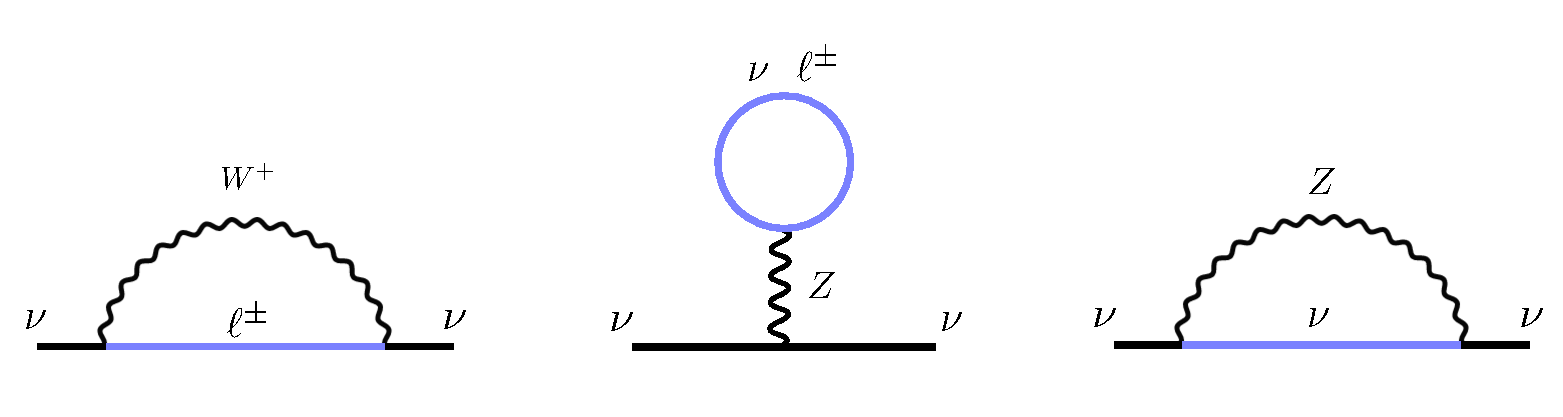
\includegraphics[width=\textwidth]{thermal_diagrams.pdf}
  \caption[Finite temperature corrections to $\Sigma$.]{Finite temperature and density corrections to the neutrino self-energy. These can be used to infer the effective matter potential for neutrinos.\label{fig:thermal_diagrams}}
\end{figure}

Now the problem reduces to computing $\Sigma$ in finite temperature field theory. For most applications of thermal mass calculations, replacing vacuum propagators by the thermal propagators from the real-time formalism is sufficient. In particular, the fermion thermal propagator of interest is
%
\begin{equation}
 S(P) = (\slashed{p} + m)\left[ \frac{1}{P^2 - m^2 +i\epsilon } + i 2\pi \delta(P^2 - m^2) f(P)\right],
\end{equation}
%
with $f(P) = \left\{ \exp\left[(|P\cdot u| - {\rm sgn}(P \cdot u) \,\mu_f)/T\right] + 1\right\}^{-1}$ is the occupational number of the fermions in the thermal bath of temperature $T$ and chemical potential $\mu_f$. Similar expressions exist for bosonic propagators. Finally, as an example, explicit computation of the tadpole self-energy contribution in \reffig{fig:thermal_diagrams} yields
%
\begin{equation}
 \Sigma = -i \frac{g^2}{16 c_\textsc{w}^2}\int \frac{\dd^4 P}{(2\pi)^4} \gamma^\mu P_L \,iS(P+K) \,\gamma^\nu \, P_L \,iD_{\mu\nu} (P),  \quad D_{\mu\nu} = \frac{-g_{\mu\nu} + \frac{P_\mu P_\nu}{M_Z^2}}{P^2 - M_Z^2 + i\epsilon}.
\end{equation}
%

By explicit computation in the rest frame of the medium, the potential for neutrinos of flavour $\alpha$ on a zero-temperature background of protons, neutrons and electrons is
%
\begin{align}
 V^e_\alpha =& -\frac{G_F}{\sqrt{2}} \left( 1-4s^2_\textsc{w} - 2\delta_{\alpha e}\right) \left( N_e - N_{\overline{e}} \right),\nonumber\\%
 V^p_\alpha =& \frac{G_F}{\sqrt{2}} \left( 1-4s^2_\textsc{w} \right) \left( N_p - N_{\overline{p}} \right),\nonumber\\%
 V^n_\alpha =& -\frac{G_F}{\sqrt{2}} \left(N_n - N_{\overline{n}} \right),
\end{align}
%
where $N_f = 2 \int \dd^3P f(P)/(2\pi)^3 $ are the number density of the background particles. For antineutrino an overall minus sign is introduced. Note the total $\nu_e$ potential is the only one where CC interactions contribute, and so it is the sole responsible for non-trivial flavour evolution in \refeq{eq:matter_evolution}. One may wonder about radiative corrections to these potentials in the SM and whether additional flavour non-universality can be achieved through the difference in charged-lepton masses. These effects, however, are known to be extremely small in the SM~\cite{Botella:1986wy}, where $\left(V_\tau - V_\mu\right)/V_e \approx 5 \times 10^{-5}$ for a neutral unpolarized medium like the Earth. 


\section{Neutrinos in the Laboratory}

To find a source of neutrinos, all we have to do is to look for environments where the weak force is prominently manifested. Natural candidates are nuclear reactors, having played a crucial role in the discovery of the neutrino. Fortunately, the list does not stop there. Abundant neutrino sources include the Sun, the atmosphere, the Big-Bang, particle accelerators and more violent astrophysical environments such as supernovae, active galactic nuclei and others. In this thesis, we will focus mostly on accelerator neutrinos.

Accelerator experiments typically produce neutrinos with energies of a few GeV to achieve $\mathcal{O}(1)$ oscillation phases $\Delta m^2_{\rm atm} L/E$ within thousands of km. Drastically different energy regimes are impractical either due to diluted fluxes at longer baselines ($\Phi \propto 1/L^2$), or due to thresholds to produce muons in CC interactions ($E_\nu > m_\ell + m_\ell^2/2 m_{\mathcal{H}}$ in reactions of the type $\nu_\ell \mathcal{H} \,\to\, \ell^\pm \mathcal{H}^\prime$). Proton beams with multi-GeV energies are used to produce neutrinos through the following steps: the protons are directed onto a dense target, the charged mesons produced in the proton-on-target collisions are focused with magnetic fields into a decay pipeline, and charged particles are absorbed further down the line. This allows the mesons to decay into neutrinos, most often through $\pi^\pm \to \overset{(-)}{\nu_\mu}\, \mu^\pm$. These experiments produce neutrinos within a wide range of energies, giving rise to wide-band beams. The shape and normalization of the neutrino flux produced are hard to model due to hadro-production and focusing uncertainties~\cite{Aliaga:2016oaz}. This comes mainly from the difficulty in describing hadron-nucleus interactions, their attenuation in propagation and, ultimately, by lack of data. In this way, the expected neutrino event rate in neutrino detectors inherits two sources of uncertainties which are difficult to disentangle: the unoscillated flux spectra and the neutrino-matter cross sections. 

For oscillation physics, however, one is only interested in disentangling uncertainties in the event rate and the effects of oscillations. One effective method to achieve this is to build near detectors, where unoscillated rate is measured, as well as far detectors, where oscillations have developed. By definition, near detectors have to be limited by the systematics of the experiment, and so require a large number of neutrino interactions. These are dominated by the processes shown in \reffig{fig:interactions_diagram} and their NC analogues. Because these processes are often subject to large nuclear effects (see below), other cleaner probes, such as neutrino-lepton scattering offer a better probe of the weak interactions in isolation. This argument will be essential when we search for \emph{stronger than weak} neutrino interactions (new interactions with 4-Fermi coupling constants with $G_X > G_F$). 
%
\begin{figure}[t]
\centering
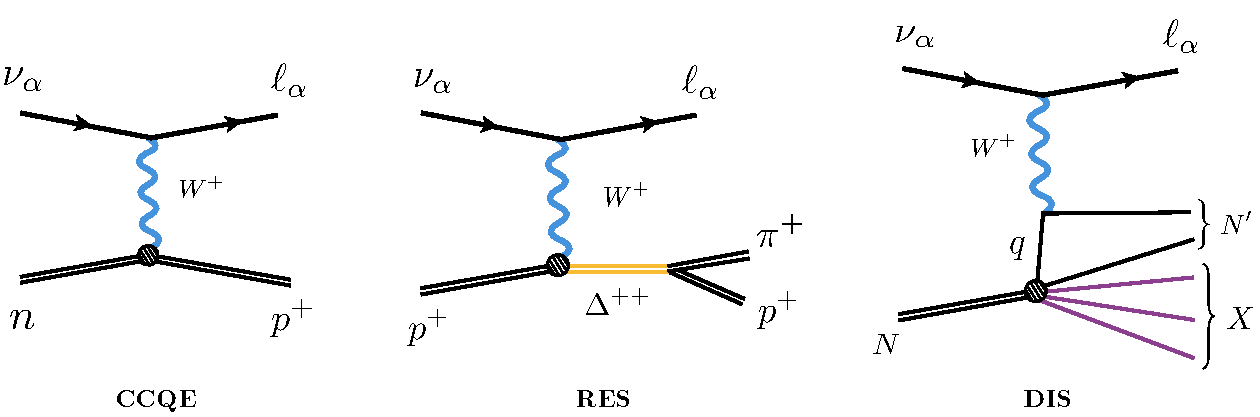
\includegraphics[width=\textwidth]{interactions.pdf}
  \caption[Neutrino nucleon interactions.]{The CC neutrino-nucleon scattering relevant for GeV neutrinos.From left to right, the CC quasi-elastic (CCQE), resonant (RES) and deep-inelastic scattering (DIS) regimes. Analogous diagrams exist for NC scattering. \label{fig:interactions_diagram}}
\end{figure}
%

\subsection{Interactions and Challenges}

Despite interacting exclusively through the weak force, when the neutrino scatters on a target nucleus, the visible final states are subject to the influence of the nuclear force. Opting for dense materials with large nuclei is preferred for oscillation physics, but as more precision is required in oscillation measurements, more control over the nuclear effects is needed. The near and far measurements of the neutrino flux helps in reducing systematics, but the neutrino flux at the near site is different from the oscillated flux at the far site, both in shape and in flavour composition. In this way, understanding how nuclear effects and neutrino cross sections depend on neutrino energy $E_\nu$ and neutrino flavour is of great importance. Let us comment on a few examples. Even in the crudest approximation for a nucleus, that of a $T=0$ Fermi gas of free protons and neutrons, nucleon final states are Pauli blocked and the occupation number of these fermions suppresses the total cross section. For realistic nuclei, these nucleons also display Fermi motion with momenta in the rest frame of the nucleus, $|p_N| \lesssim 250$ MeV, that are comparable to the incoming neutrino energy. On their way out of the nucleus, struck nucleons may also exchange EM charge, knock-out additional particles or be absorbed by the nuclear medium. 
%
\begin{figure}[t]
\centering
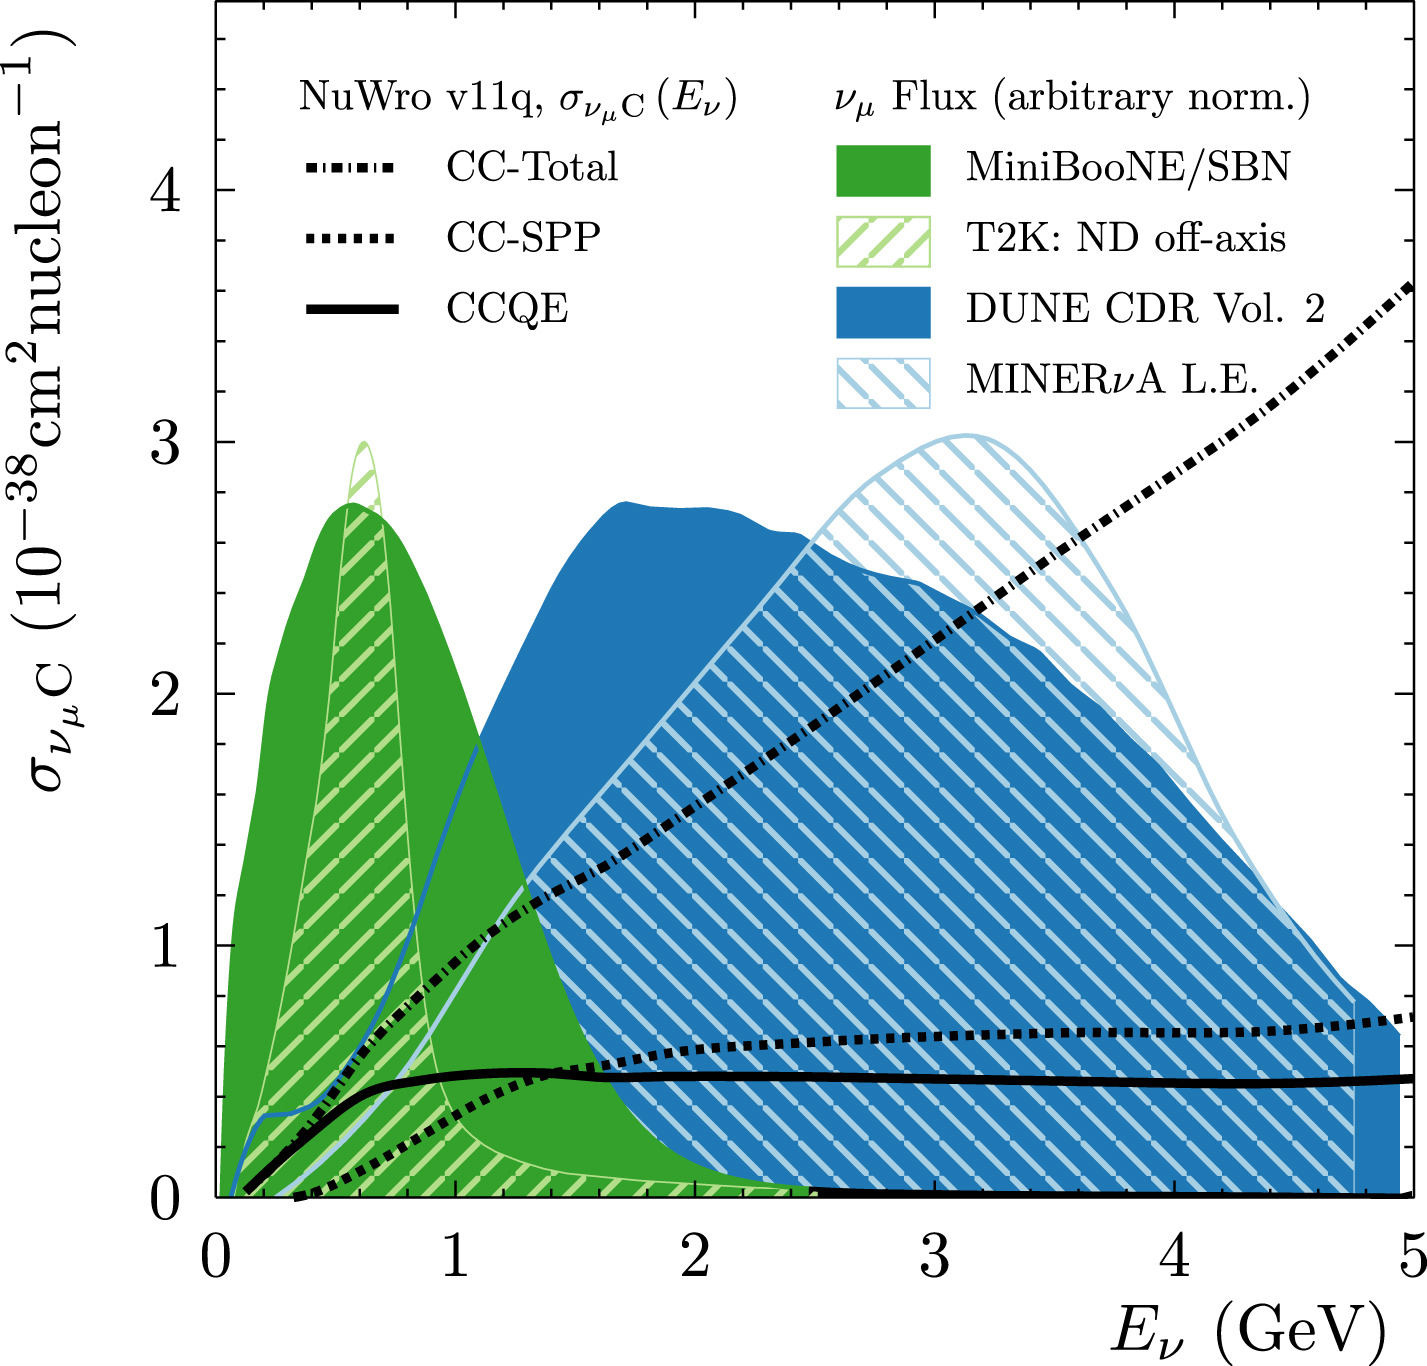
\includegraphics[width=0.45\textwidth]{cross_sections.jpg}
  \caption[Neutrino cross sections and the neutrino flux of current and future accelerator experiments.]{Figure from Ref.~\cite{Betancourt:2018bpu} showing the NuWro prediction for $\nu_\mu-^{12}C$ cross section per nucleon for {CCQE} scattering, CC single pion production (CC-SPP, dominated by {RES} diagrams), and for total CC scattering (including {DIS}). Overlaid are some of the neutrino fluxes of MINER$\nu$A, MiniBooNE, SBN, T2K off-axis and a projection for DUNE. \label{fig:compare_cross_sections}}
\end{figure}
%
The importance of nuclear effects is perhaps most famously illustrated by the measurement of the CC quasi-elastic (CCQE) process by the MiniBooNE~\cite{AguilarArevalo:2010zc} experiment. MiniBooNE is an accelerator experiment where a neutrino flux with an average energy of $\langle E_\nu \rangle \approx 800 $ MeV is directed towards a detector filled with mineral oil, made mostly of $CH$ molecules. A disagreement of $20\%$ was observed between the MC prediction and the data, unless the axial mass $M_A$ was set to be $\approx1.32$ GeV, much larger than the world-average of $M_A = 1.03 \pm 0.02$ GeV. This was later understood as a missing contribution from two-particle two-hole meson exchange currents (where the neutrino interacts with a nucleon pair, rather than with an individual nucleon), shown to be as large as $30\%$ of the CCQE cross section used by the experiment~\cite{Nieves:2011yp}.

The most common interactions of neutrino with the nucleons in the detector are displayed in \reffig{fig:interactions_diagram}. Below $\lesssim1$ GeV, CCQE scattering is most common, but at larger energies the resonant (RES) contributions start to become more important. The decay of the intermediate resonance is also affected by the nuclear medium and this has to be implemented in a nuclear model-dependent way, such as in the so called microscopical models. Another approach is that of macroscopic models, where one makes use of hypotheses such as the partially conserved axial current (PCAC) to relate the neutrino cross sections with the meson-nucleus cross section~\footnote{PCAC is the result of the spontaneous breaking of the chiral symmetry $SU(2)_L \times SU(2)_R$ in the quark sector. Because this symmetry is explicitly broken by quark masses, the pion is massive (although quite light compared to the $\eta$ meson, for instance) and therefore the pseudo-Golstone boson of the theory.}. The PCAC relation for neutrino scattering holds only for the $q^2 = (k_1 - k_2)^2 \to 0$ limit, where the incoming neutrino momenta $k_1$ is parallel to the outgoing lepton momenta $k_2$. This is a good approximation of the cross section at large energies, but breaks down at low energies, where it is very often used~\cite{Hernandez:2009vm}. For larger neutrino energies $E_\nu\gtrsim 3$ GeV, the deep-inelastic scattering (DIS) regime start to dominate. Here, the cross section calculations are much more reliable, although nuclear effects are still in place (see Ref.~\cite{Mousseau:2016snl}, for instance). Past neutrino scattering experiments such as NuTeV, CCFR and CHARM operated at neutrino energies in the tens and hundreds of GeV, and provided the most precise measurements of the neutrino DIS cross sections to date. All the processes we just discussed are now  implemented in several neutrino event generators, the most popular being GENIE~\cite{Andreopoulos:2009rq}, GiBUU~\cite{Buss:2011mx}, NEUT~\cite{Hayato:2002sd} and NuWro~\cite{Juszczak:2005zs}. Different neutrino-nucleus cross section models are implemented in these generators, but one typically relies on tuning to pre-existing data to make predictions. For illustration, in \reffig{fig:compare_cross_sections} we show the NuWro predictions for CC cross sections, overlaid on neutrino fluxes in current and future accelerator experiments.





